% !TEX program = pdflatex
% Informe final: Más brecha que efecto (PISA 2025, Argentina)
% Compilación: latexmk -pdf informe_final.tex   (ver paper/README.md)
\documentclass[11pt,a4paper]{article}

% ---------- Codificación, idioma y tipografía ----------
\usepackage[T1]{fontenc}
\usepackage[utf8]{inputenc}
\usepackage[spanish,es-tabla,es-nodecimaldot,es-noshorthands]{babel}
\usepackage[sc]{mathpazo}
\linespread{1.06}
\usepackage[final]{microtype}
\usepackage{csquotes}
\usepackage[htt]{hyphenat}
\emergencystretch=2.5em

% ---------- Página ----------
\usepackage[a4paper,top=2.4cm,bottom=2.4cm,left=2.5cm,right=2.5cm,headheight=14pt]{geometry}
\usepackage{fancyhdr}
\pagestyle{fancy}
\fancyhf{}
\fancyhead[L]{\small\textsc{Urday Quiroga, Cordero y Sanchez}}
\fancyhead[R]{\small\textit{Más brecha que efecto: IA y desigualdad en PISA 2025}}
\fancyfoot[C]{\small\thepage}
\renewcommand{\headrulewidth}{0.3pt}

% ---------- Matemática, tablas, figuras ----------
\usepackage{amsmath,amssymb,bm}
\usepackage{booktabs,tabularx,array,threeparttable}
\usepackage{graphicx}
\usepackage[dvipsnames]{xcolor}
\usepackage{tikz}
\usetikzlibrary{positioning,arrows.meta,calc}
\usepackage{enumitem}
\setlist{itemsep=1pt,topsep=3pt}
\setlength{\tabcolsep}{4.5pt}
\usepackage[font=small,labelfont=bf,labelsep=period,justification=justified,singlelinecheck=false]{caption}
\usepackage{titlesec}
\definecolor{azul}{HTML}{1F5FA8}
\definecolor{gristexto}{HTML}{555555}
\titleformat{\section}{\large\bfseries\color{azul}}{\thesection.}{0.6em}{}
\titleformat{\subsection}{\normalsize\bfseries}{\thesubsection.}{0.5em}{}
\titleformat{\subsubsection}[runin]{\normalsize\itshape}{}{0em}{}[.]
\titlespacing*{\section}{0pt}{1.6\baselineskip}{0.6\baselineskip}
\titlespacing*{\subsection}{0pt}{1.1\baselineskip}{0.4\baselineskip}

% ---------- Bibliografía ----------
\usepackage[backend=bibtex,style=authoryear,maxcitenames=2,maxbibnames=8,giveninits=true,
            uniquename=init,doi=true,url=true,isbn=false,natbib=true]{biblatex}
\addbibresource{referencias.bib}
\renewcommand*{\bibfont}{\small}

\usepackage[colorlinks=true,linkcolor=azul,citecolor=azul,urlcolor=azul,
            pdftitle={Más brecha que efecto: nivel socioeconómico, uso de chatbots de inteligencia artificial y rendimiento escolar en Argentina (PISA 2025)},
            pdfauthor={Nazareno Urday Quiroga, Juan Ignacio Cordero, Matias Sanchez}]{hyperref}

% ---------- Macros ----------
\newcommand{\var}[1]{\texttt{#1}}
\newcommand{\nb}[1]{\texttt{\small notebooks/#1}}
\newcommand{\arch}[1]{\texttt{\small #1}}
\newcommand{\E}{\operatorname{E}}
\newcommand{\V}{\widehat{V}}
\newcommand{\ee}{\operatorname{ee}}
\newcommand{\pp}{\,p.p.}
\newcommand{\ic}[2]{IC\,95\,\%: #1 a #2}
\DeclareMathOperator*{\argmin}{arg\,min}
\makeatletter\newcommand{\filas}[1]{\@@input tablas/#1.tex }\makeatother % \input expandible, compatible con booktabs

\begin{document}

\thispagestyle{plain}
\vspace*{-0.8cm}
\noindent{\color{azul}\rule{\textwidth}{1.2pt}}\par\vspace{0.45cm}
\noindent{\LARGE\bfseries Más brecha que efecto\par}
\vspace{0.3cm}
\noindent{\large Nivel socioeconómico, uso de chatbots de inteligencia artificial y rendimiento escolar en Argentina: evidencia de PISA~2025\par}
\vspace{0.4cm}
\noindent{\large Nazareno Urday Quiroga, Juan Ignacio Cordero y Matias Sanchez}\par
\vspace{0.3cm}
\noindent{\color{azul}\rule{\textwidth}{0.4pt}}\par\vspace{0.35cm}

\noindent\small
\textbf{Resumen.} Con los microdatos de PISA~2025 para Argentina (11.092 estudiantes, 412 escuelas) se estima cómo se asocian el nivel socioeconómico y el uso de chatbots de inteligencia artificial (IA) con el rendimiento, usando el peso final, los 80 pesos replicados y los 10 valores plausibles. Cada unidad del índice ESCS se asocia con 30,6 puntos más en ciencias (\ic{26,3}{34,8}) y el cuartil superior supera al inferior en 82,4 puntos. Entre quienes respondieron, el cuartil superior usa IA semanal o diariamente entre 13 y 17 puntos porcentuales más. Sin ajustar, el uso frecuente frente a ninguno se asocia con $+$28,4 puntos al investigar un tema, $+$26,6 al ayudar a aprender y $+$18,8 al resumir, pero no al redactar borradores. Al ajustar por ESCS, sexo y grado, la asociación cae un 58\,\%, a 4,0 puntos por punto de frecuencia (\ic{1,1}{6,9}). El 29\,\% de quienes recibieron las preguntas de IA no las respondió y rinde 66,0 puntos menos. Dentro de una misma escuela, la pendiente socioeconómica del uso es menos de la mitad que en el total. Los datos muestran una brecha de uso alineada con la desigualdad de origen y situada sobre todo entre escuelas; no permiten atribuir efectos a la IA.

\smallskip\noindent\textbf{Palabras clave:} PISA~2025; inteligencia artificial generativa; desigualdad educativa; nivel socioeconómico; no respuesta; Argentina.

\par\normalsize
\vspace{0.25cm}\noindent{\color{azul}\rule{\textwidth}{0.4pt}}\par

% =====================================================================
\section{El problema}\label{sec:problema}

Los chatbots de IA entraron al trabajo escolar antes de que hubiera datos poblacionales sobre quién los usa. El debate público se plantea en términos de efecto ---si la IA \enquote{mejora} o \enquote{empeora} el aprendizaje---, pero esa pregunta depende de otra previa: \emph{quiénes} la usan y \emph{con qué frecuencia}. En Argentina, como en la mayoría de los sistemas educativos, el rendimiento está fuertemente asociado al origen social \parencite{sirin2005}. Si el uso de IA también lo está, comparar a quienes la usan con quienes no la usan mezcla la herramienta con las condiciones de quienes acceden a ella, y lo que parece un efecto de la IA puede ser, en buena medida, la desigualdad que ya existía. La literatura sobre brecha digital anticipa exactamente eso: una vez extendido el acceso, la desigualdad se traslada a los usos \parencite{hargittai2002}. Y la evidencia experimental disponible indica que el resultado depende del modo de uso: en un experimento con estudiantes secundarios, un asistente sin restricciones perjudicó el desempeño posterior sin la herramienta \parencite{bastani2025}.

PISA~2025 permite por fin mirar el problema con datos representativos. Su cuestionario pregunta con qué frecuencia cada estudiante usa chatbots de IA para cuatro actividades escolares ---resumir un texto, investigar un tema nuevo, redactar borradores y ayudar a aprender---, preguntas que no existían en el archivo de 2022. En los mismos estudiantes se observan el rendimiento, el nivel socioeconómico y los pesos muestrales.

\paragraph{Pregunta.} ¿Cómo se asocian el nivel socioeconómico y la frecuencia de uso de chatbots de IA con el rendimiento de los estudiantes argentinos, y cuánto de la asociación entre IA y rendimiento sobrevive cuando se tiene en cuenta el origen social?

\paragraph{Qué se encontró.} Cinco resultados, que el resto del artículo desarrolla:
\begin{enumerate}[label=\textbf{\arabic*.},leftmargin=1.6em]
\item El gradiente socioeconómico del rendimiento es grande: 82 puntos de ciencias separan al cuartil superior del inferior.
\item El uso frecuente de IA sigue el mismo gradiente: 13 a 17 puntos porcentuales más en el cuartil superior, en las cuatro actividades.
\item La ventaja bruta de quienes usan IA con frecuencia (19 a 28 puntos) se reduce un 58\,\% al ajustar por contexto y solo se sostiene para investigar y para ayudar a aprender; para redactar borradores nunca aparece.
\item Casi tres de cada diez estudiantes no respondieron las preguntas de IA, y son los de menor rendimiento (66 puntos menos): lo que PISA puede decir sobre IA en Argentina vale para un grupo desplazado hacia arriba.
\item La brecha de uso se localiza sobre todo entre escuelas: dentro de una misma escuela es menos de la mitad.
\end{enumerate}

\noindent Las hipótesis H1 a H5 y sus parámetros se fijaron antes de calcular; HC1 surgió al preparar los datos y HC2 a HC4 se plantearon después de ver los primeros resultados y se registraron antes de estimarlas (\arch{docs/bitacora.md}). Todo lo que sigue son asociaciones: el diseño es transversal y no identifica efectos causales.

% =====================================================================
\section{Datos y método}\label{sec:metodo}

\paragraph{Datos.} Archivo de uso público del cuestionario del estudiante de PISA~2025 \parencite{oecd2025db}, registros de Argentina: 11.092 estudiantes de 15 años escolarizados en 412 escuelas. El rendimiento se mide con los diez valores plausibles de ciencias (matemática y lectura como contraste); el contexto, con el índice de estatus económico, social y cultural (ESCS), dividido en cuartiles ponderados relativos a Argentina ($Q_1$ a $Q_4$); el uso de IA, con cuatro ítems $A_{ik}\in\{1,\dots,5\}$ (1 = nunca o casi nunca; 5 = todos o casi todos los días). Se define \emph{uso frecuente} como semanal o diario ($A_{ik}\ge4$), \emph{ocasional} como anual o mensual ($A_{ik}\in\{2,3\}$) y la \emph{frecuencia media} $\bar A_i$ como el promedio de los cuatro ítems. Los controles son sexo y grado relativo al modal.

\paragraph{Muestras.} No se imputó ningún dato; cada análisis usa los casos completos que requiere (figura~\ref{fig:flujo}). El faltante en los ítems de IA es casi enteramente no respuesta (código 99), no un salto de cuestionario, y es de \enquote{todo o nada}: 7.475 estudiantes respondieron los cuatro ítems, 3.141 ninguno y 476 algunos.

\begin{figure}[t]
\centering
\begin{tikzpicture}[
  caja/.style={draw=azul, rounded corners=2pt, line width=0.5pt, align=center, font=\small, inner sep=4pt, text width=4.4cm},
  excl/.style={draw=gray!60, rounded corners=2pt, line width=0.4pt, align=left, font=\footnotesize, inner sep=4pt, text width=3.6cm, text=gristexto},
  fl/.style={-{Stealth[length=5pt]}, line width=0.5pt, draw=azul}]
\node[caja] (a) {Estudiantes de Argentina\\ \textbf{$n=11.092$} (412 escuelas)};
\node[caja, below=0.95cm of a] (b) {Con ESCS válido\\ \textbf{$n=9.808$} (88,4\,\%)\\ \emph{H1; HC1 ajustada}};
\node[caja, below=0.95cm of b] (c) {Con ESCS y los cuatro ítems de IA\\ \textbf{$n=7.191$} (64,8\,\%)\\ \emph{H2--H5; HC2--HC4}};
\node[excl, right=3.1cm of $(a.south)!0.5!(b.north)$] (e1) {Sin ESCS: 1.284};
\node[excl, right=3.1cm of $(b.south)!0.5!(c.north)$] (e2) {Sin los cuatro ítems de IA: 2.617};
\node[caja, left=0.8cm of b, text width=4.3cm, font=\footnotesize] (d) {{\small Bloque de IA administrado}\\ {\small\textbf{$n=10.566$}}\\ (excluye 526 no administrados)\\ respondieron los cuatro: 7.475\\ no los completaron: 3.091\\ {\small\emph{HC1 sin ajustar}}};
\draw[fl] (a) -- (b);
\draw[fl] (b) -- (c);
\draw[fl, draw=gray!70] ($(a.south)!0.5!(b.north)$) -- (e1);
\draw[fl, draw=gray!70] ($(b.south)!0.5!(c.north)$) -- (e2);
\draw[fl] (a.west) -| (d.north);
\end{tikzpicture}
\caption{Muestras analíticas. Ningún registro se elimina; cada análisis usa los casos con las variables que necesita.}\label{fig:flujo}
\end{figure}

\paragraph{Estimación.} PISA tiene un muestreo estratificado por conglomerados y entrega el rendimiento como valores plausibles, no como puntajes \parencite{mislevy1992}. Cada estadístico $\hat\theta$ (media, diferencia de medias o coeficiente de mínimos cuadrados ponderados) se calcula con el peso final $\bm{w}$ para cada valor plausible $m=1,\dots,M$ ($M=10$) y se repite con cada uno de los $G=80$ pesos replicados $\bm{w}^{(g)}$. La varianza muestral usa replicación repetida balanceada con el factor de Fay $k$ \parencite{judkins1990} y se combina con la varianza entre valores plausibles mediante las reglas de \textcite{rubin1987}:
\begin{align}
\V_m&=\frac{1}{G(1-k)^2}\sum_{g=1}^{G}\bigl(\hat\theta(\bm{w}^{(g)},m)-\hat\theta(\bm{w},m)\bigr)^2, \label{eq:fay}\\
\V(\hat\theta)&=\frac1M\sum_{m=1}^{M}\V_m+\Bigl(1+\frac1M\Bigr)\frac{1}{M-1}\sum_{m=1}^{M}\bigl(\hat\theta(\bm{w},m)-\hat\theta\bigr)^2, \label{eq:var}
\end{align}
con $\hat\theta=\tfrac1M\sum_m\hat\theta(\bm{w},m)$. Se usó $k=0{,}5$, el valor documentado por la OCDE para ciclos anteriores \parencite{oecd2009manual}; la documentación técnica de 2025 es provisional y no permitió confirmarlo. Las estimaciones puntuales no dependen de $k$. Los intervalos son $\hat\theta\pm1{,}96\,\ee(\hat\theta)$ y los valores $p$ bilaterales usan la referencia normal.

\paragraph{Modelos.} La asociación condicional entre IA y rendimiento (H4) y su variación con el ESCS (H5) se estiman con
\begin{equation}\label{eq:h4}
Y_i=\beta_0+\beta_A \bar A_i+\beta_E\,\text{ESCS}_i+\beta_S\,\text{sexo}_i+\beta_D\,\text{grado}_i\;\bigl[+\beta_{AE}\,\bar A_i\times\text{ESCS}_i\bigr]+\varepsilon_i ,
\end{equation}
con las variables centradas cuando se incluye la interacción. Para HC4 se compara la pendiente de $\bar A$ sobre el ESCS en el total ($b_T$) con la pendiente dentro de la escuela ($b_W$), obtenida restando a cada variable la media ponderada de su escuela. Ambas cumplen la identidad
\begin{equation}\label{eq:descomp}
b_T=\rho\,b_B+(1-\rho)\,b_W,\qquad 0\le\rho\le1,
\end{equation}
donde $b_B$ es la pendiente entre medias de escuela y $\rho$ la fracción de la variabilidad del ESCS que ocurre entre escuelas. De~\eqref{eq:descomp} se sigue que la parte de $b_T$ debida al componente entre escuelas es al menos $1-b_W/b_T$.

\paragraph{Decisión.} Un resultado se considera \emph{compatible con una asociación} si $p<\alpha$; en caso contrario, la evidencia es \emph{insuficiente}, lo que no equivale a ausencia de asociación. Se usa $\alpha=0{,}05$, con corrección de Bonferroni en los ocho contrastes de H3 ($p<0{,}00625$) y en las tres hipótesis HC2--HC4 ($p<0{,}0167$). Como referencia de magnitud, las diferencias se comparan con la brecha de 82,4 puntos entre cuartiles extremos de ESCS.

% =====================================================================
\section{Resultados}\label{sec:resultados}

Todas las cifras provienen de \arch{reports/tables/}; los cuadros se generan por programa a partir de esas tablas (\arch{paper/tablas.py}).

\subsection{Dos gradientes socioeconómicos: rendimiento y uso de IA}
Cada unidad adicional de ESCS se asocia con 30,6 puntos más en ciencias (\ic{26,3}{34,8}), 29,3 en matemática y 28,2 en lectura (cuadro~\ref{tab:h1h2}; figura~\ref{fig:h1h2}a). Las medias de ciencias por cuartil son 367, 382, 402 y 449 puntos: la diferencia entre extremos es de 82,4 puntos (\ic{70,2}{94,5}) y más de la mitad se concentra en el salto al cuartil superior (47 puntos entre $Q_3$ y $Q_4$).

El uso de IA sigue el mismo gradiente. Entre los 7.191 estudiantes con ESCS y los cuatro ítems respondidos, la proporción que usa IA semanal o diariamente es mayor en el cuartil superior en todas las actividades: 16,9\pp{} al investigar, 15,8\pp{} al resumir, 14,7\pp{} al ayudar a aprender y 13,3\pp{} al redactar borradores (figura~\ref{fig:h1h2}b). La frecuencia media es 0,49 puntos mayor en la escala de 1 a 5 (\ic{0,36}{0,62}).

\begin{table}[t]
\caption{Asociación del ESCS con el rendimiento (H1) y con el uso de IA (H2).}\label{tab:h1h2}
\small
\begin{threeparttable}
\begin{tabularx}{\textwidth}{@{}Xrrrrr@{}}
\toprule
Parámetro & $n$ & Estimación & EE & IC 95\,\% & $p$ \\
\midrule
\filas{tab_h1_h2}
\bottomrule
\end{tabularx}
\begin{tablenotes}\footnotesize
\item Pendientes en puntos PISA por unidad de ESCS. $Q_4-Q_1$: cuartil superior menos inferior de ESCS. EE: error estándar; p.p.: puntos porcentuales. Uso frecuente: semanal o diario.
\end{tablenotes}
\end{threeparttable}
\end{table}

\begin{figure}[t]
\centering
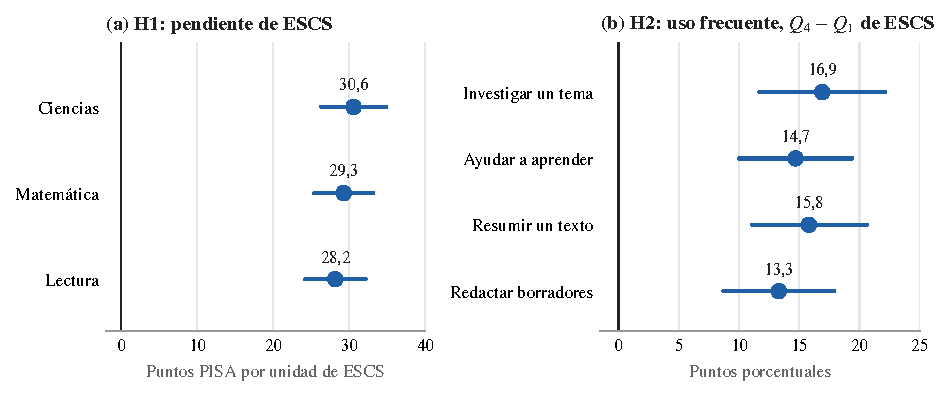
\includegraphics[width=\textwidth]{figuras/fig_h1_h2.pdf}
\caption{(a)~Pendiente del ESCS sobre el rendimiento. (b)~Diferencia entre cuartiles extremos de ESCS en la proporción que usa IA semanal o diariamente. Puntos: estimación; líneas: IC\,95\,\%. En todas las figuras, punto lleno azul: el intervalo excluye el cero; punto hueco gris: lo incluye.}\label{fig:h1h2}
\end{figure}

\subsection{La ventaja bruta de quienes usan IA}
Sin ajustar, quienes usan IA con frecuencia superan en ciencias a quienes nunca la usan en tres de las cuatro actividades (cuadro~\ref{tab:h3}; figura~\ref{fig:h3}): investigar un tema ($+$28,4 puntos; \ic{17,6}{39,3}), ayudar a aprender ($+$26,6; \ic{17,2}{36,0}) y resumir un texto ($+$18,8; \ic{9,4}{28,1}). Las tres superan el umbral de Bonferroni y equivalen al 35\,\%, 32\,\% y 23\,\% de la brecha entre cuartiles extremos de ESCS. Para redactar borradores la diferencia no se distingue de cero ($+$7,1; \ic{$-$3,0}{17,2}).

La relación no es gradual: el uso ocasional no se diferencia del no uso en ninguna actividad, y en redactar borradores la estimación es incluso negativa ($-$8,5; \ic{$-$18,0}{0,9}). La asociación se concentra en el extremo superior de la escala de frecuencia.

\begin{table}[t]
\caption{H3: diferencias de medias en ciencias según la frecuencia de uso de IA, sin ajustar.}\label{tab:h3}
\small
\begin{threeparttable}
\begin{tabularx}{\textwidth}{@{}Xrrrrr@{}}
\toprule
Contraste y actividad & $n$ & Diferencia & EE & IC 95\,\% & $p$ \\
\midrule
\filas{tab_h3}
\bottomrule
\end{tabularx}
\begin{tablenotes}\footnotesize
\item $^{\ast}$ Supera el umbral de Bonferroni para ocho contrastes ($p<0{,}00625$).
\end{tablenotes}
\end{threeparttable}
\end{table}

\begin{figure}[t]
\centering
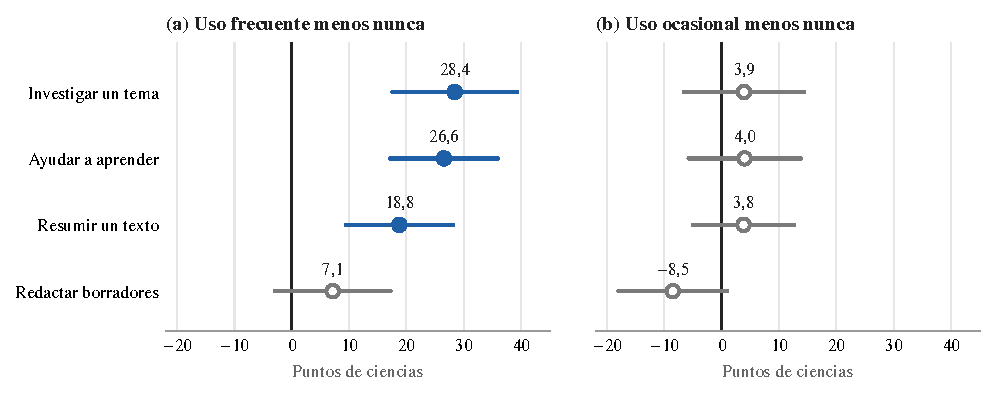
\includegraphics[width=\textwidth]{figuras/fig_h3.pdf}
\caption{H3: diferencia de medias en ciencias respecto de quienes nunca usan IA, sin ajustar. (a)~Uso semanal o diario. (b)~Uso anual o mensual.}\label{fig:h3}
\end{figure}

\subsection{Qué queda al tener en cuenta el origen social}
Este es el resultado central. Sin controles, cada punto adicional de frecuencia media se asocia con 9,48 puntos más en ciencias. Al incorporar el ESCS el coeficiente baja a 5,02 (un 47\,\% menos) y con ESCS, sexo y grado a 4,03 (\ic{1,14}{6,92}; $p=0{,}0063$): una reducción total del 58\,\% (cuadro~\ref{tab:h4h5}; figura~\ref{fig:h4}a). Más de la mitad de la ventaja bruta acompañaba al contexto, no al uso.

Lo que queda es modesto: recorrer toda la escala de frecuencia, de 1 a 5, equivale bajo linealidad a unos 16 puntos, una quinta parte de la brecha entre cuartiles extremos de ESCS. Y no es uniforme entre actividades (figura~\ref{fig:h4}b): la asociación condicional se mantiene para investigar un tema (5,24; \ic{2,61}{7,88}) y ayudar a aprender (5,55; \ic{3,22}{7,88}), desaparece para resumir (1,60; \ic{$-$0,65}{3,84}) ---que mostraba una ventaja bruta de 19 puntos--- y es nula para redactar borradores ($-$0,64). El patrón distingue los usos en que la herramienta interviene en la comprensión de aquel en que produce el texto.

No hay evidencia suficiente de que la asociación cambie con el nivel socioeconómico (H5): la interacción es $+$2,42 (\ic{$-$0,31}{5,15}; $p=0{,}082$).

\begin{table}[t]
\caption{H4 y H5: coeficiente de la frecuencia de uso de IA sobre ciencias (puntos por punto de la escala 1--5; $n=7.191$).}\label{tab:h4h5}
\small
\begin{threeparttable}
\begin{tabularx}{\textwidth}{@{}Xrrrrr@{}}
\toprule
Modelo y regresor & $n$ & Coeficiente & EE & IC 95\,\% & $p$ \\
\midrule
\filas{tab_h4_h5}
\bottomrule
\end{tabularx}
\begin{tablenotes}\footnotesize
\item \enquote{Ajustado}: controla ESCS, sexo y grado (ecuación~\ref{eq:h4}). $^{\dagger}$ Del análisis de sensibilidad.
\end{tablenotes}
\end{threeparttable}
\end{table}

\begin{figure}[t]
\centering
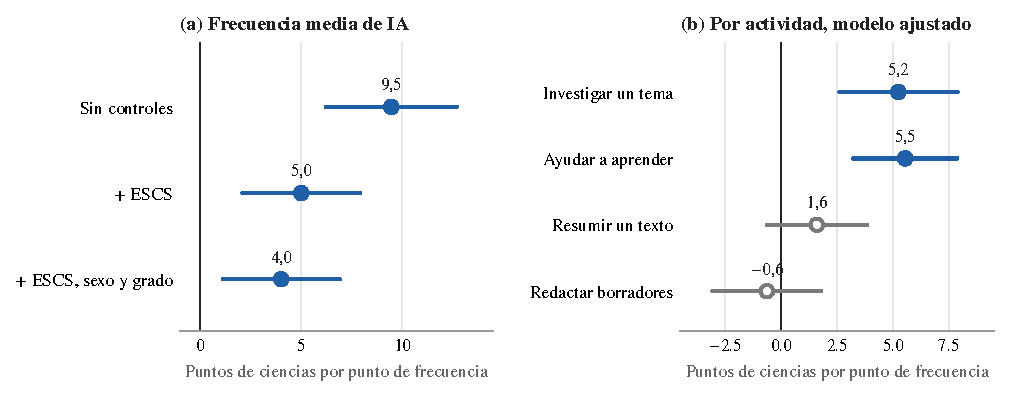
\includegraphics[width=\textwidth]{figuras/fig_h4.pdf}
\caption{H4. (a)~El coeficiente de la frecuencia media de IA se reduce al incorporar controles. (b)~Coeficiente de cada actividad en el modelo ajustado.}\label{fig:h4}
\end{figure}

\subsection{Quiénes no respondieron}
De los 10.566 estudiantes a quienes se administró el bloque de IA, 3.091 (29\,\%) no completaron los cuatro ítems. No son un grupo al azar: quienes sí respondieron obtienen 66,0 puntos más en ciencias (\ic{57,7}{74,2}), el 80\,\% de la brecha entre cuartiles extremos de ESCS. Ajustando por ESCS la diferencia sigue siendo de 53,8 puntos (\ic{46,4}{61,2}): el origen social explica una parte menor (cuadro~\ref{tab:hc}; figura~\ref{fig:hc}a).

La consecuencia es directa. Todo lo que PISA~2025 permite decir sobre IA en Argentina describe a los estudiantes que respondieron, que rinden bastante más que el resto. Si la no respuesta se relaciona con el propio uso de IA ---algo que los datos no permiten saber---, las brechas reales pueden ser distintas de las estimadas.

\subsection{A quién llega la IA y dónde se produce la brecha}
Tres hipótesis exploratorias afinan el cuadro (cuadro~\ref{tab:hc}; figura~\ref{fig:hc}).

\emph{El uso es mayor entre quienes más rinden} (HC3). El cuartil de mayor rendimiento en ciencias usa IA semanal o diariamente 16,6\pp{} más que el de menor rendimiento (\ic{11,3}{22,0}). Es la misma asociación de la sección anterior leída al revés, y recuerda que su dirección es indeterminada: puede que quienes rinden más adopten más la herramienta.

\emph{La brecha se produce sobre todo entre escuelas} (HC4). La pendiente del ESCS sobre la frecuencia media de uso es 0,185 en el total (\ic{0,139}{0,231}) y 0,080 al comparar estudiantes de una misma escuela (\ic{0,026}{0,134}). La pendiente intraescuela es el 43\,\% de la total; por la identidad~\eqref{eq:descomp}, al menos el 57\,\% de la pendiente total corresponde al componente entre escuelas. La desigualdad de uso depende más de a qué escuela se asiste que de las diferencias entre compañeros. La proporción es un cociente de estimaciones puntuales, sin error estándar propio.

\emph{La diferencia es de cuánto, no de para qué} (HC2). Un índice que resta la frecuencia de redactar al promedio de investigar y aprender no difiere entre cuartiles extremos de ESCS ($+$0,082; \ic{$-$0,030}{0,194}). No hay evidencia de que los estudiantes de distinto origen usen la IA para cosas distintas.

\begin{table}[t]
\caption{Hipótesis complementarias y exploratorias.}\label{tab:hc}
\small
\begin{threeparttable}
\begin{tabularx}{\textwidth}{@{}Xrrrrr@{}}
\toprule
Parámetro & $n$ & Estimación & EE & IC 95\,\% & $p$ \\
\midrule
\filas{tab_hc}
\bottomrule
\end{tabularx}
\begin{tablenotes}\footnotesize
\item $^{\ast}$ Supera el umbral de Bonferroni para tres hipótesis ($p<0{,}0167$). $T$: promedio de investigar y aprender menos redactar. Pendientes de HC4 en puntos de la escala 1--5 por unidad de ESCS.
\end{tablenotes}
\end{threeparttable}
\end{table}

\begin{figure}[t]
\centering
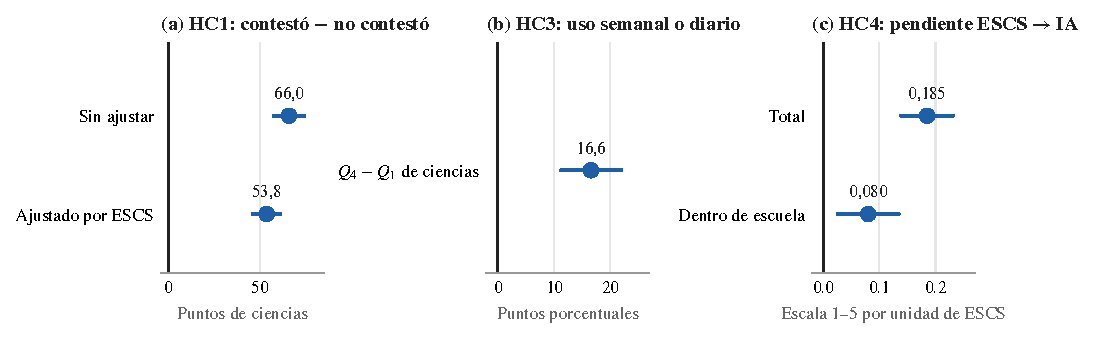
\includegraphics[width=\textwidth]{figuras/fig_exploratorias.pdf}
\caption{(a)~HC1: diferencia en ciencias entre quienes respondieron los ítems de IA y quienes no. (b)~HC3: diferencia en uso semanal o diario entre cuartiles extremos de rendimiento. (c)~HC4: pendiente del ESCS sobre la frecuencia de uso, total y dentro de la escuela.}\label{fig:hc}
\end{figure}

\subsection{Robustez}
El signo y el orden entre actividades se mantienen en todas las variantes examinadas (figura~\ref{fig:sens}). El coeficiente ajustado es similar en matemática (4,19) y lectura (3,31), con el índice de uso de IA en la escuela que calcula PISA (3,61; $p=0{,}030$) y al incluir respuestas parciales (4,15). Comparar el uso diario con el no uso reproduce el patrón de H3: $+$26,8 para ayudar a aprender, $+$21,0 para investigar, $+$12,5 para resumir y un resultado no concluyente para redactar. Haber usado IA \emph{alguna vez} no se asocia con el rendimiento ($+$6,1; \ic{$-$6,5}{18,7}): el 92\,\% de la muestra analítica la usó alguna vez, de modo que lo que diferencia a los estudiantes es la frecuencia, no el acceso. Lo que más mueve la magnitud son los controles.

Con criterios más exigentes el panorama se ordena. Bajo una corrección de Bonferroni sobre las 46 estimaciones del proyecto ($p<0{,}0011$) se sostienen H1, H2, las tres diferencias brutas de H3, la no respuesta y HC3; no la superan el coeficiente ajustado de H4 ni la pendiente intraescuela de HC4. Con una referencia $t$ de 80 grados de libertad en lugar de la normal no cambia ningún veredicto (\arch{paper/verificacion\_cifras.txt}).

\begin{figure}[t]
\centering
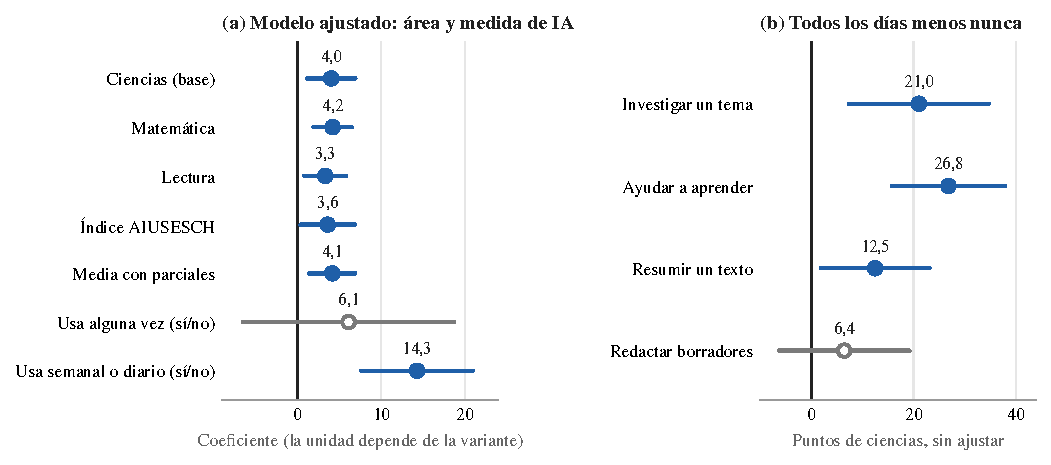
\includegraphics[width=\textwidth]{figuras/fig_sensibilidad.pdf}
\caption{Robustez. (a)~Coeficiente ajustado según el área y la medida de uso de IA (las unidades difieren entre variantes). (b)~Diferencia en ciencias entre uso diario y ningún uso, sin ajustar.}\label{fig:sens}
\end{figure}

% =====================================================================
\section{Discusión}\label{sec:discusion}

\paragraph{Más brecha que efecto.} Los datos sostienen con firmeza dos gradientes paralelos ---rendimiento y uso de IA--- ordenados por el origen social, y una asociación entre IA y rendimiento que se reduce a menos de la mitad en cuanto se la compara entre estudiantes de contexto similar. El residuo de 4 puntos por punto de frecuencia admite tres lecturas que estos datos no distinguen: características no observadas del estudiante o de la escuela, causalidad inversa (HC3 muestra la misma asociación con los roles invertidos) o algún beneficio de ciertos usos. Es además el resultado confirmatorio más frágil ante criterios estrictos de multiplicidad.

\paragraph{El tipo de actividad importa como descripción.} Investigar y ayudar a aprender conservan una asociación positiva en todas las especificaciones; redactar borradores, en ninguna. Es coherente con la evidencia experimental de que el modo de uso es decisivo \parencite{bastani2025}, pero aquí no puede leerse como que unos usos \enquote{sirven} y otros no: también puede reflejar qué estudiantes eligen cada uso.

\paragraph{La no respuesta es un resultado, no solo un límite.} Que el 29\,\% no haya respondido y rinda 66 puntos menos significa que la población para la que PISA describe el uso de IA en Argentina excluye de manera desproporcionada a los estudiantes más rezagados, precisamente aquellos sobre quienes más interesa saber.

\paragraph{La escuela como unidad de la brecha.} Que la pendiente socioeconómica del uso caiga a menos de la mitad dentro de una misma escuela sitúa la desigualdad en la segregación entre establecimientos. Para la política educativa, la escuela aparece como el nivel donde intervenir.

\paragraph{Límites.} (i)~El diseño es transversal: ningún coeficiente es un efecto. (ii)~Los resultados sobre IA valen para quienes respondieron; no se reponderó ni se imputó. (iii)~El uso es autodeclarado y se reduce a la frecuencia de cuatro actividades; el ESCS es un índice relativo, no ingreso. (iv)~Los controles son tres; con más covariables el coeficiente de H4 podría reducirse más. (v)~El factor de Fay de 2025 no está confirmado: si fuera otro, cambiarían los errores estándar, no las estimaciones. (vi)~Los cortes de los cuartiles de ESCS no se recalcularon en cada réplica. (vii)~El análisis no se contrastó con software de encuestas de terceros.

% =====================================================================
\section{Conclusión}\label{sec:conclusion}

En Argentina, según PISA~2025, el uso de chatbots de IA está socialmente estratificado: lo usan con más frecuencia los estudiantes de mayor nivel socioeconómico, de mayor rendimiento y de ciertas escuelas. La ventaja de rendimiento de quienes usan IA con frecuencia existe en bruto, pero el 58\,\% desaparece al tener en cuenta el contexto, y lo que resta es pequeño, limitado a dos actividades y sin interpretación causal. A la vez, casi tres de cada diez estudiantes ---los de menor rendimiento--- quedan fuera de la fotografía por no haber respondido.

La respuesta a la pregunta es asimétrica: PISA permite afirmar con solidez \emph{quién} usa la IA y permite afirmar muy poco sobre \emph{qué produce}. Los pasos siguientes son caracterizar la no respuesta, vincular la brecha entre escuelas con las características de los establecimientos y abordar la pregunta causal con diseños longitudinales o experimentales.

\paragraph{Datos y código.} El código, las tablas y las figuras están en el repositorio \texttt{nazareno-urday/pisa-analysis-argentina} de GitHub. Los microdatos se obtienen de la OCDE \parencite{oecd2025db}.

\printbibliography[title={Referencias}]

\end{document}
